\documentclass{article}
\usepackage[utf8]{inputenc}

\title{Assignment 5}
\author{Jahnavi Pragada,EE19B049}
\date{\today}

\usepackage{natbib}
\usepackage{graphicx}
\usepackage{amsmath}
\usepackage{listings}

\begin{document}

\maketitle

\section*{Abstract}
We wish to solve for the currents in a resistor. The currents depend on the shape of the resistor.

\section*{Introduction}
A  cylindrical wire is soldered to the middle of a copper plate and its voltage is held at 1 Volt.  One side of the plate is grounded, while the remaining are floating. The plate is 1 cm by 1 cm in size.\newline
We shall use these equations:\newline
The Continuity Equation:
\begin{equation}
    \nabla \cdot \vec{j} = - \frac{\partial\rho}{\partial t}
\end{equation}
Ohms Law:
\begin{equation}
    \vec{j} = \sigma\vec{E}
\end{equation}
The above equations along with the definition of potential as the negative gradient of Field give:
\begin{equation}
    \nabla^2 \phi =  \frac{1}{\rho}\frac{\partial\rho}{\partial t}
\end{equation}
For DC Currents, RHS of equation (3) is 0. Hence:
\begin{equation}
    \nabla^2 \phi =  0
\end{equation}

\section*{Assignment 5}
\subsection*{Defining Parameters}

\lstset{language=Python}
\lstset{label={lst:code_direct}}
\lstset{basicstyle=\footnotesize}
\begin{lstlisting}
if(len(sys.argv)==5):
    Nx=int(sys.argv[1])
    Ny=int(sys.argv[2])
    radius=int(sys.argv[3])  
    Niter=int(sys.argv[4])
else:
    Nx=25 # size along x
    Ny=25 # size along y
    radius=8 #radius of central lead
    Niter=1500 #number of iterations to perform
    
\end{lstlisting}

\subsection*{Initializing Potential }
We start by creating an zero 2-D array of size Nx x Ny,then a list of coordinates lying within the radius is generated and these points are initialized to 1. The graph of potential is plotted using contour function in figure 1.
\begin{lstlisting}
phi=np.zeros((Nx,Ny),dtype = float)
x=np.linspace(-0.5,0.5,Nx)
y=np.linspace(-0.5,0.5,Ny)
Y,X=np.meshgrid(y,x)
ii=np.where(X**2+Y**2<(0.35)**2)
phi[ii]=1.0
plt.xlabel("X")
plt.ylabel("Y")
plt.contourf(X,Y,phi)
plt.plot(x_c,y_c,'ro')
plt.colorbar()
plt.show()
\end{lstlisting}

\begin{figure}[h!]
\centering
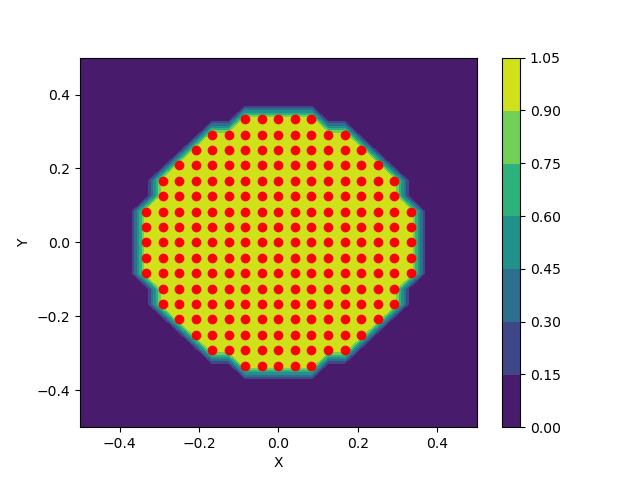
\includegraphics[scale=0.7]{Figure_1_5.png}
\caption{Initial potential}
\label{Initial potential}
\end{figure}



\subsection*{Performing Iterations}
\subsubsection*{Updating Potential}
We use Equation(4) to do this.But Equation (4) is a differential equation. We need to first convert it to a difference equation as all of our code is in discrete domain.
We write it as :
\begin{equation}
    \phi_{i,j} = 0.25*(\phi_{i-1,j} + \phi_{i+1,j} + \phi_{i,j+1} + \phi_{i,j-1})
\end{equation}
\begin{lstlisting}
def update_phi(phi,phiold):
    phi[1:-1,1:-1]=0.25*(phiold[1:-1,0:-2]+ phiold[1:-1,2:]+ 
                         phiold[0:-2,1:-1]+ phiold[2:,1:-1])
    return phi
\end{lstlisting}

\subsubsection*{Applying Boundary Conditions}
The bottom boundary is grounded. The other 3 boundaries have a normal potential of 0
\begin{lstlisting}
def boundary(phi):
    phi[1:-1,0]=phi[1:-1,1] # Left Boundary
    phi[1:-1,Nx-1]=phi[1:-1,Nx-2] # Right Boundary
    phi[0,1:-1]=phi[1,1:-1] # Top Boundary
    phi[Ny-1,1:-1]=0
    phi[ii]=1.0
    return phi
\end{lstlisting}
\subsubsection*{Calculating error and running iterations}
\begin{lstlisting}
for k in range(Niter):
    phiold = phi.copy()
    phi = update_phi(phi,phiold)
    phi = boundary(phi)
    err[k] = np.max(np.abs(phi-phiold))
\end{lstlisting}

\subsubsection*{Plotting the errors}
We will plot the errors on semi-log and log-log plots. We note that the error falls really slowly and this is one of the reasons why this method of solving the Laplace equation is discouraged. Semilog and loglog plots of error are figure 2,3

\begin{lstlisting}
plt.figure(num=2)
plt.title("Error on a semilog plot")
plt.xlabel("No of iterations")
plt.ylabel("Error")
plt.semilogy((np.asarray(range(Niter))+1),err)
plt.semilogy((np.asarray(range(Niter))+1)[::50],err[::50],'ro')
plt.show()

\end{lstlisting}

\begin{figure}[h!]
\centering
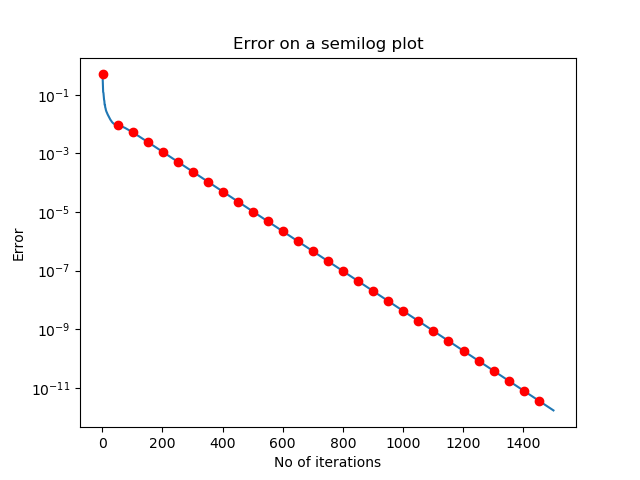
\includegraphics[scale=0.6]{Figure_2_5.png}
\caption{Semilog plot of error}
\label{Semilog plot of error}
\end{figure}

\begin{figure}[h!]
\centering
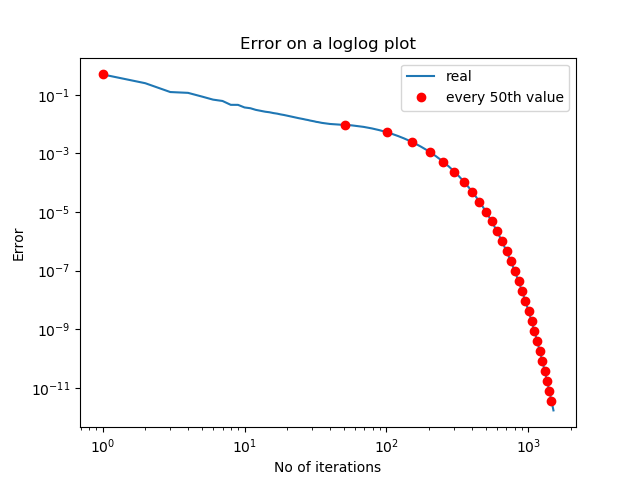
\includegraphics[scale=0.6]{Figure_3_5.png}
\caption{Loglog plot of error}
\label{Loglog plot of error}
\end{figure}



\subsection*{Fitting the error}
We note that the error is decaying exponentially for higher iterations.I have plotted 2 fits. One considering all the iterations(fit1) and another without considering the first 500 iterations. There is very little difference between the two fits. Figure 4,5 are plots of best fit
\begin{lstlisting}

def fit(y,Niter,lastn=0):
    log_err = np.log(err)[-lastn:]
    X = np.vstack([(np.arange(Niter)+1)[-lastn:],np.ones(log_err.shape)]).T
    log_err = np.reshape(log_err,(1,log_err.shape[0])).T
    return s.lstsq(X, log_err)[0]


def plot_error(err,Niter,a,a_,b,b_):
    plt.title("Best fit for error on a loglog scale")
    plt.xlabel("No of iterations")
    plt.ylabel("Error")
    x = np.asarray(range(Niter))+1
    plt.loglog(x,err)
    plt.loglog(x[::100],np.exp(a+b*np.asarray(range(Niter)))[::100],'ro')
    plt.loglog(x[::100],np.exp(a_+b_*np.asarray(range(Niter)))[::100],'go')
    plt.legend(["errors","fit1","fit2"])
    plt.show()

b,a = fit(err,Niter)
b_,a_ =fit(err,Niter,500)
plot_error(err,Niter,a,a_,b,b_)
\end{lstlisting}

\begin{figure}[h!]
\centering
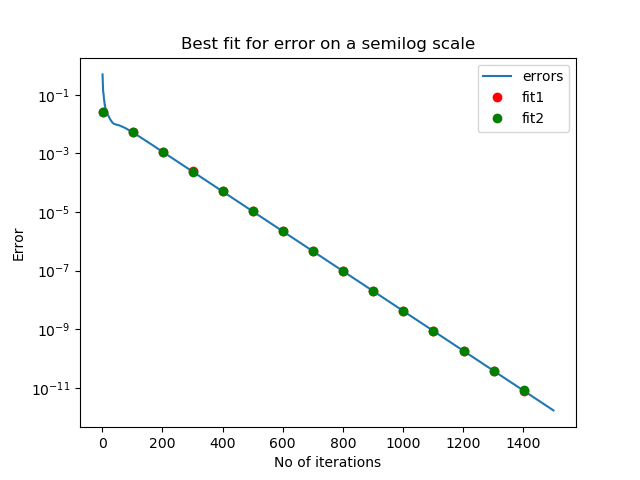
\includegraphics[scale=0.7]{Figure_4_5.png}
\caption{Best fit Semilog plot of error}
\label{Best fit Semilog plot of error}
\end{figure}


\begin{figure}[h!]
\centering
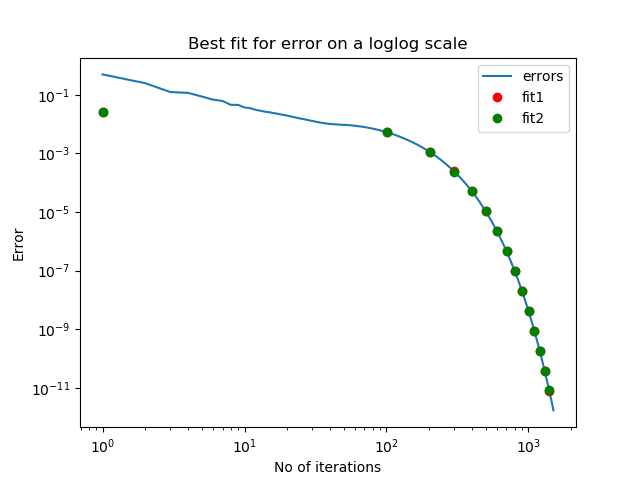
\includegraphics[scale=0.5]{Figure_5_5.png}
\caption{Best fit Loglog plot of error}
\label{Best fit Loglog plot of error}
\end{figure}


\subsection*{Plotting $\phi$}
3D Surface plot of potential in figure 6. 2D contour plot in figure 7
\begin{lstlisting}
fig1=plt.figure(4)     # open a new figure
ax=p3.Axes3D(fig1) # Axes3D is the means to do a surface plot
plt.title('The 3-D surface plot of the potential')
surf = ax.plot_surface(Y, X, phi.T, rstride=1, cstride=1, cmap=plt.cm.jet)
plt.show()
\end{lstlisting}
\begin{figure}[h!]
\centering
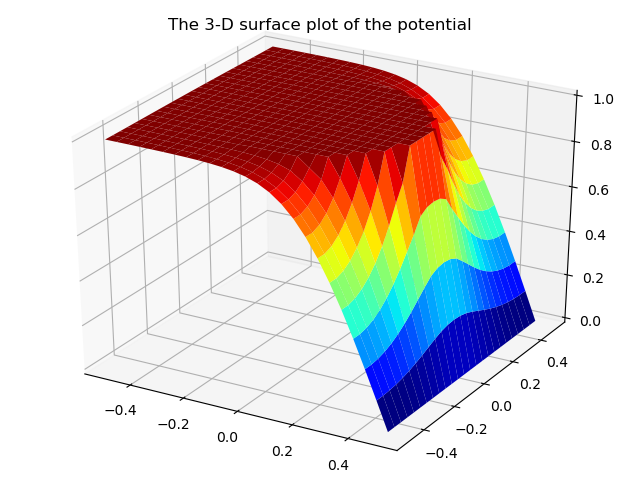
\includegraphics[scale=0.5]{Figure_8_5.png}
\caption{Surface Potential plot}
\label{Surface Potential plot}
\end{figure}
\begin{lstlisting}
plt.title("2D Contour plot of potential")
plt.xlabel("X")
plt.ylabel("Y")
plt.contourf(Y,X[::-1],phi)
plt.colorbar()
plt.show()
\end{lstlisting}




\begin{figure}[h!]
\centering
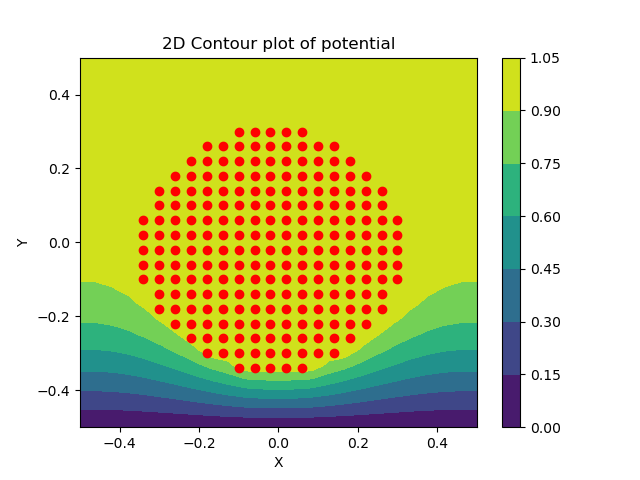
\includegraphics[scale=0.5]{Figure_7_5.png}
\caption{Contour Potential plot}
\label{Contour Potential plot}
\end{figure}

\subsection*{Finding and Plotting $J$}
\begin{equation}
    J_{x,ij} = 0.5*(\phi_{i,j-1} - \phi_{i,j+1})
\end{equation}
\begin{equation}
    J_{y,ij} = 0.5*(\phi_{i-1,j} - \phi_{i+1,j})
\end{equation}
\begin{lstlisting}
Jx,Jy = (1/2*(phi[1:-1,0:-2]-phi[1:-1,2:]),1/2*(phi[:-2,1:-1]-phi[2:,1:-1]))

plt.title("Vector plot of current flow")
plt.quiver(Y[1:-1,1:-1],-X[1:-1,1:-1],-Jx[:,::-1],-Jy)
x_c,y_c=np.where(X**2+Y**2<0.35**2)
plt.plot((x_c-Nx/2)/Nx,(y_c-Ny/2)/Ny,'ro')
plt.show()
\end{lstlisting}







\begin{figure}[h!]
\centering
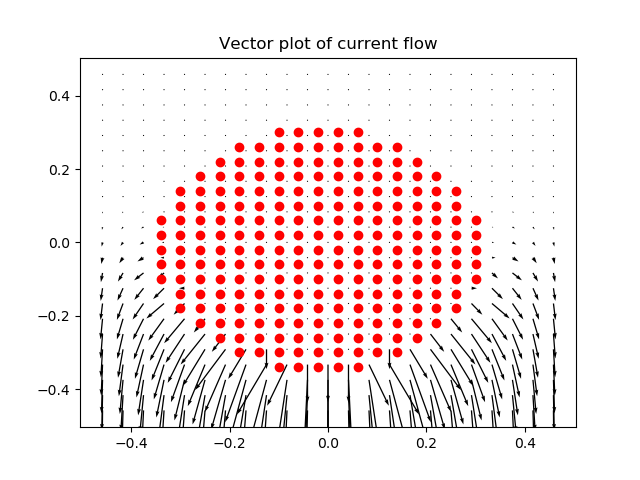
\includegraphics[scale=0.7]{Figure_9_5.png}
\caption{Current Plot}
\label{Current plot}
\end{figure}
\end{document}

